\documentclass[a4paper, 11pt, twocolumn]{article}
\usepackage[margin=0.8in]{geometry}
\usepackage{xcolor}
\usepackage{graphicx} %package to manage images
\graphicspath{ {./images/} }

\title{A2-01 Further Sequential Logic Systems}
\author{Revision Sheet}
\date{}

\usepackage{fancyhdr}
\pagestyle{fancy}
\fancyhead{} % clear all header fields
\renewcommand{\headrulewidth}{0pt} % no line in header area
\fancyfoot{} % clear all footer fields
\renewcommand{\footrulewidth}{0.4pt}
\fancyfoot[C]{\thepage} % page number in centre of the page
\fancyfoot[R]{\footnotesize Thomas Boxall \\ Images from WJEC E-BOok} % right hand footer has author name on top line and images reference on bottom line
\fancyfoot[L]{\footnotesize A2-01 Further Sequential Logic Systems \\ Revision sheet} % left hand footer has title of document on top line and 'Revision Sheet' on bottom line

\begin{document}
\maketitle
\thispagestyle{fancy}
\noindent This topic only contains Synchronous counters.
\section{Introduction}
Synchronous counters based on D flip-flops differ from ripple counters and dedicated synchronous counters as they can produce any sequence of output signals, where as ripple counters can only count up or down in binary; the clock signals are connected together and so receive clock pulses at exactly the same time and the logic gates generate appropriate signals at the data inputs of each stage.\\
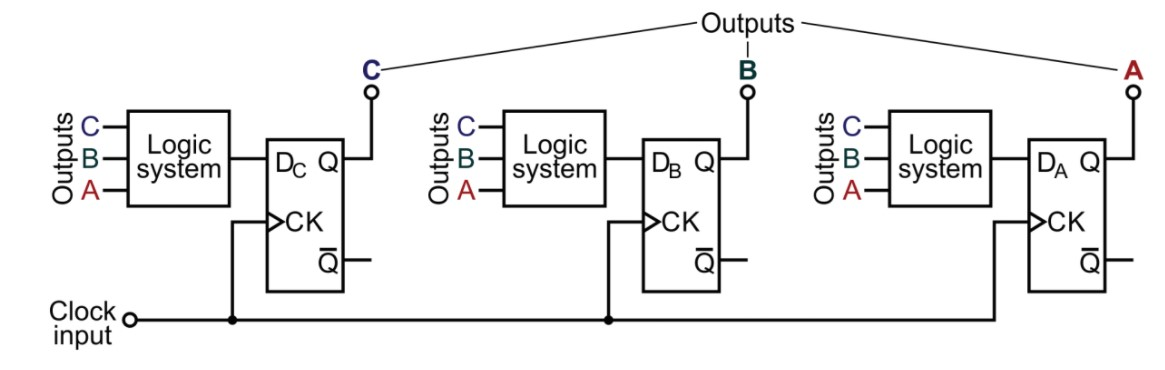
\includegraphics[width=0.4\textwidth]{basicDiagram.jpg}\\

\section{Designing a Synchronous Counter}
\subsection{Step 1}
Formalise the required sequence of output states. In this example, it will be shown as a truth table. In a truth table, on the same line as the current binary sequence, also show the next binary sequence. \\
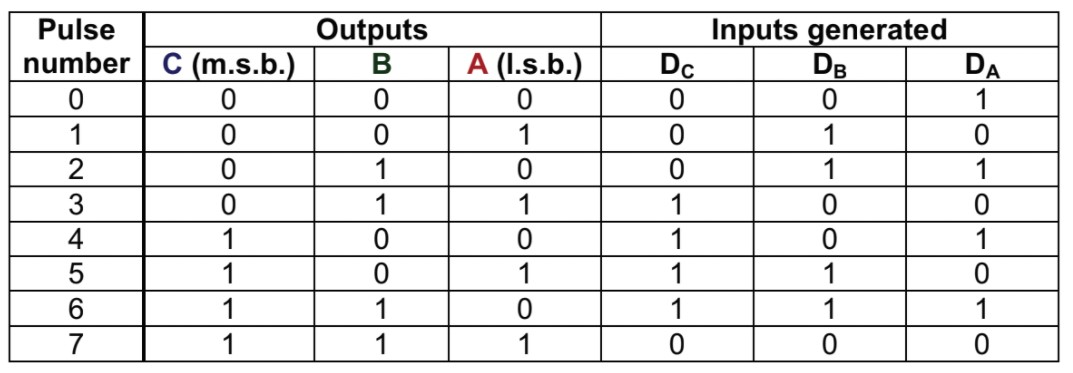
\includegraphics[width=0.4\textwidth]{step1.jpg}\\

\subsection{Step 2}
This step is to derive boolean logic expressions for each of the inputs to the flip flops. In this example, they are as follows.\newline
$D_{C}=C \cdot \bar{B} + B \cdot (C \bigoplus A)$\newline
$D_B = D \bigoplus A$\newline
$D_A = \bar{A}$

\subsection{Step 3}
We can then draw the circuit diagram of the counter.\\
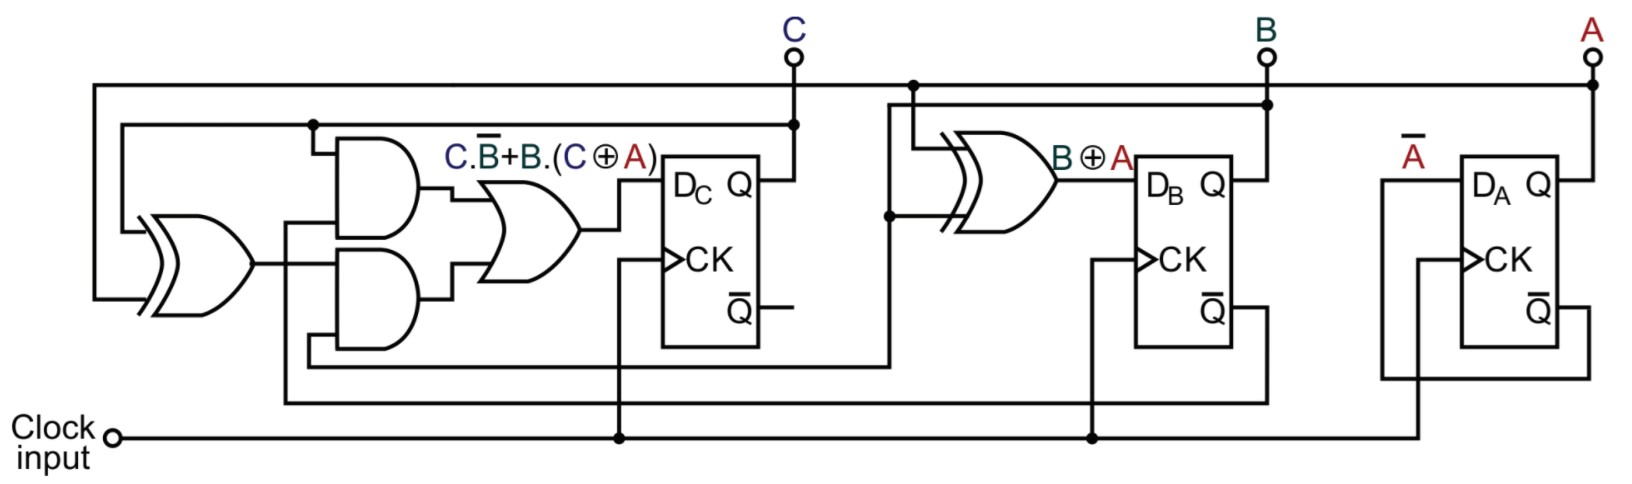
\includegraphics[width=0.4\textwidth]{step2.jpg}

\section{Other Parts to design}
In the example above, there were a number of stages which weren't covered. These include
\subsection{State Diagrams}
This is a state diagram. It shows how each of the states progress from one to another.\\
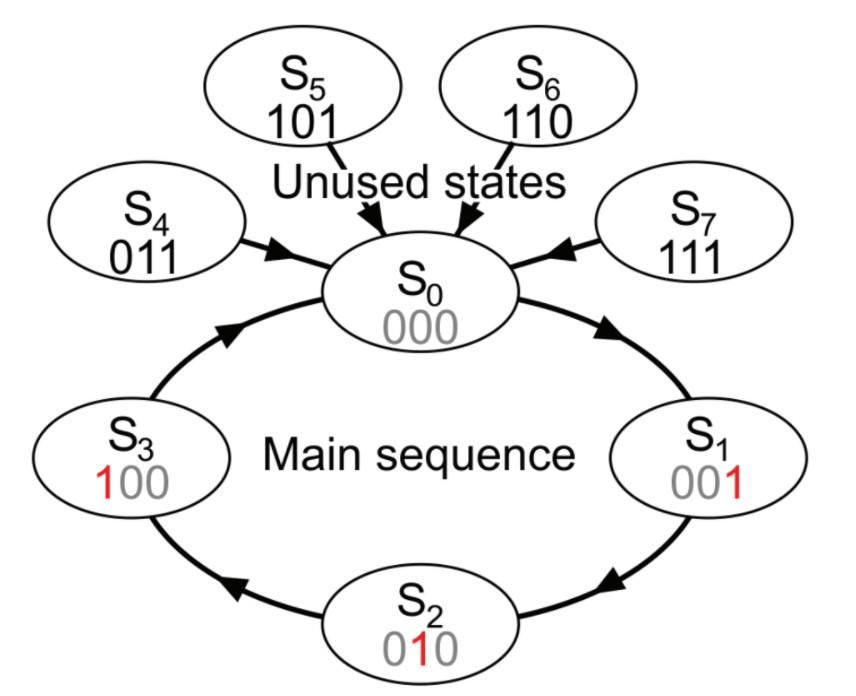
\includegraphics[width=0.4\textwidth]{state.jpg}

\subsection{Don't care states}
Don't care states are states which aren't used in the main sequence. We can use this to our advantage because they can be used when simplifying the boolean expression to make the expression as simple as possible. They are written in as 'X' and can be treated as a '1' or '0' depending on the best place to group bits together on a Karnaugh Map.

\section{Stuck states}
Sometimes, when designing a synchronous counter, there are states which don't feed into the main states loop. These might form a smaller loop off to the side. They are called stuck states and are bad.\newline
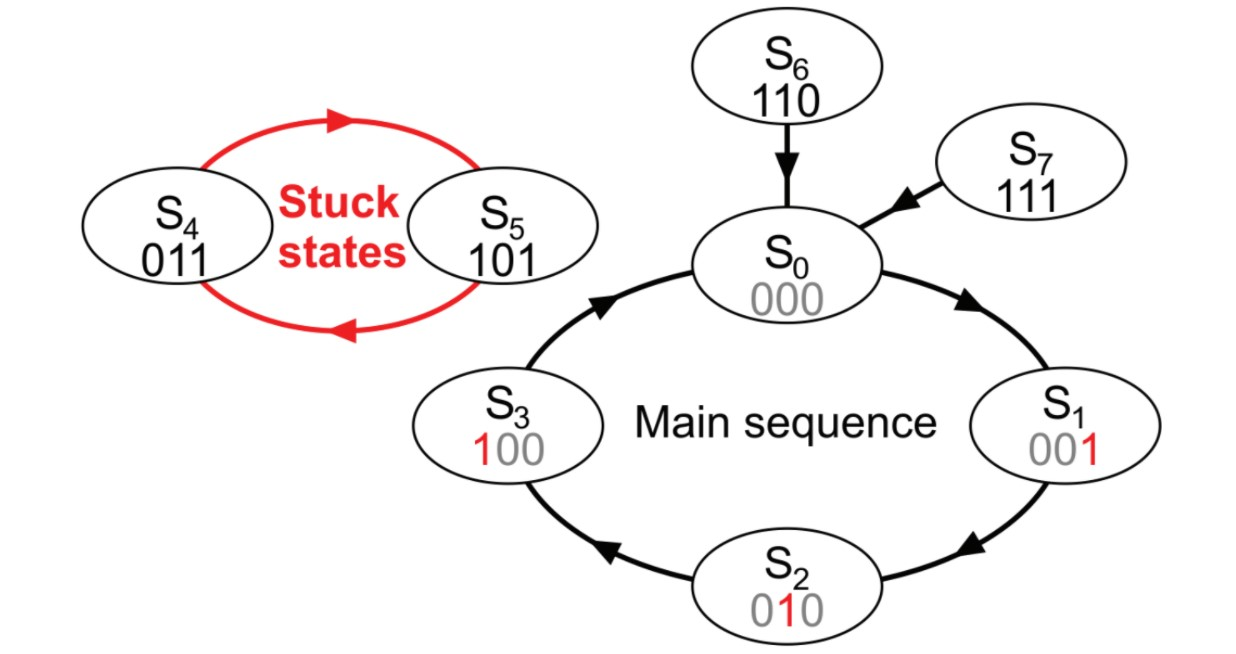
\includegraphics[width=0.4\textwidth]{stuckStates.jpg}

\end{document}